
\section{Website Operations and Management}
This section provides an overview of the website in the classic view mode. The classic view provides a user-friendly interface for navigating and managing various aspects of the website.

\subsection{Overview of Classic View}
The classic view of the website consists of several sections, each represented by specific UI elements. Below are the key sections and their functionality:
\begin{figure}[htbp]
  \centering
  \itshape
  % Replace the path below with your actual image path
  \setlength{\fboxrule}{1pt}  % Border thickness
  \setlength{\fboxsep}{3pt}   % Space between image and border
  % \framebox[0.8\linewidth]{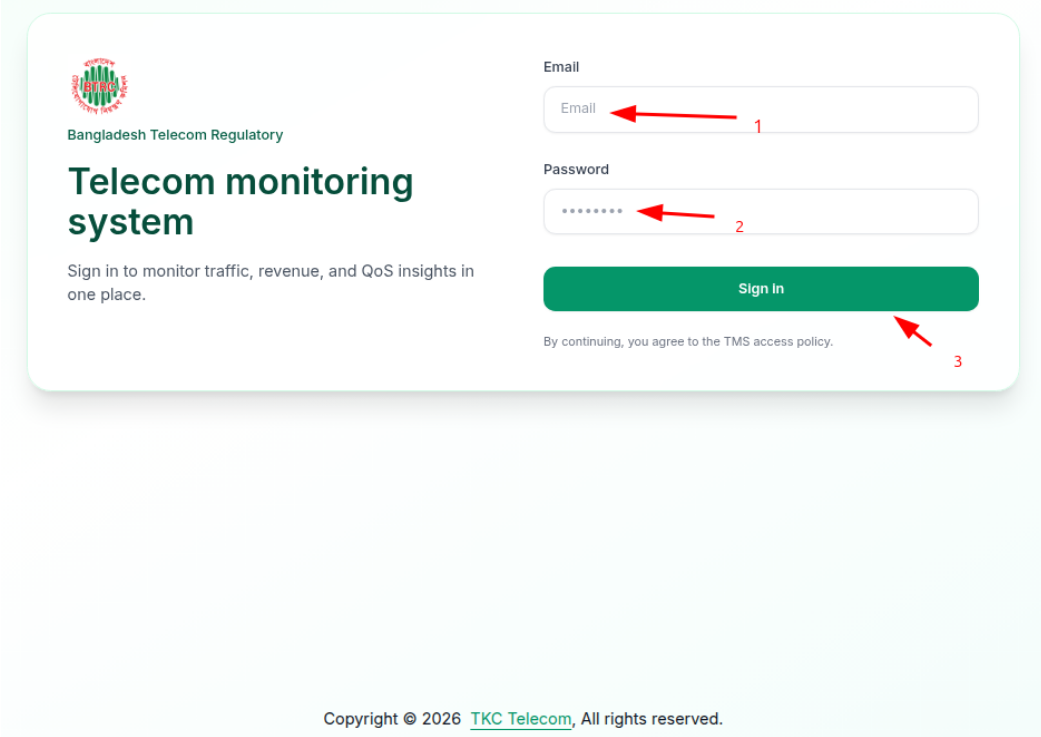
\includegraphics[width=0.8\linewidth]{img/login/login.png}}
  \colorbox{gray!20}{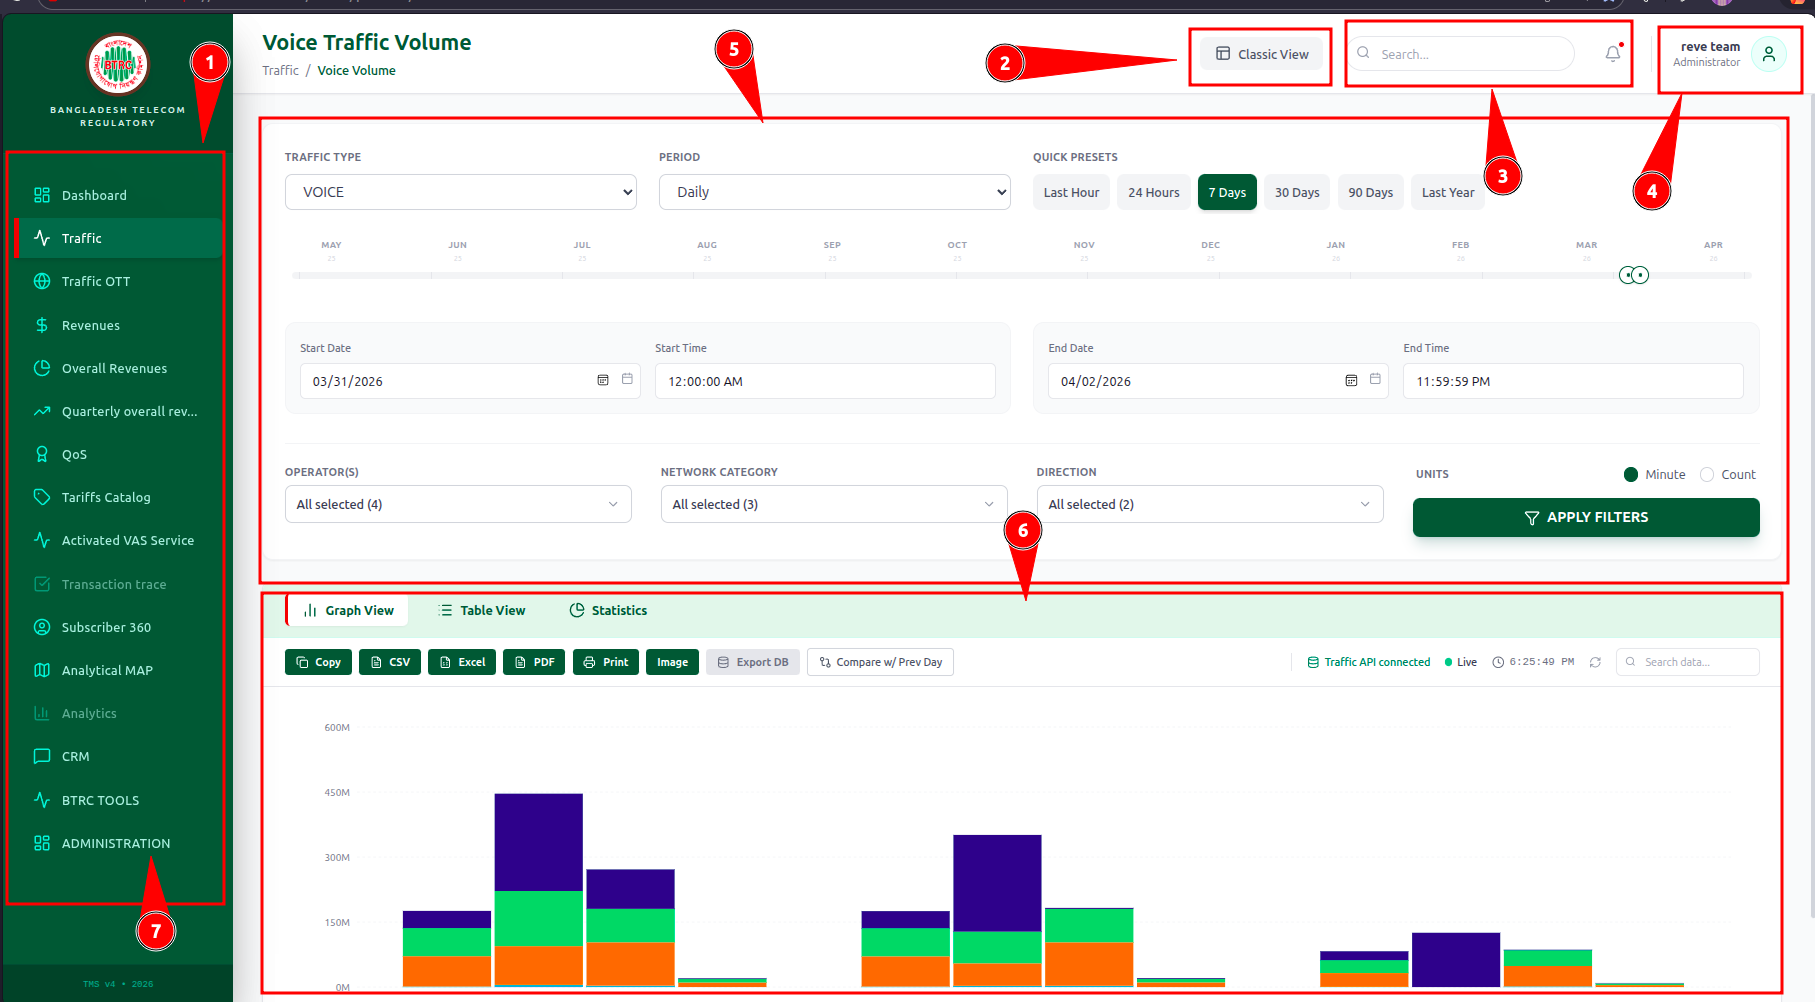
\includegraphics[width=1\linewidth]{img/websiteOperations/webOparation.png}}
  \caption{Classic View Overview}
  \label{fig:classic-view-overview}
\end{figure}
\begin{itemize}
  \item \textbf{Menu Bar (Pointer 1)}: This is the main navigation panel on the left-hand side of the website. It allows users to access various sections like Dashboard, Traffic, Revenues, QoS, Tariffs Catalog, and others.
  \item \textbf{Classic and Modern View Switch Button (Pointer 2)}: This button allows the user to switch between the classic and modern view of the website. The user can toggle between these views to get a different perspective or user interface.
  \item \textbf{Search on this Page (Pointer 3)}: The search bar enables users to quickly search for specific data or reports on the page.
  \item \textbf{Profile of User (Pointer 4)}: This section displays the logged-in user's profile. It shows their name, role (Administrator or other), and other personal details. Users can access settings and log out from this section.
  \item \textbf{Custom Search (Pointer 5)}: This allows users to apply specific filters or search criteria. It includes options like time range, operators, network categories, and direction for traffic data. Users can enter custom search queries to view the relevant data.
  \item \textbf{User Custom Search Results (Pointer 6)}: Once the filters are applied, the results are displayed here. The data is shown in a graphical format (bar charts, etc.) depending on the selected filters.
  \item \textbf{Administration Section (Pointer 7)}: This section is only visible to users with administrative privileges. Non-admin users will not have access to this section.
\end{itemize}

\subsection{Classic View Description}
The classic view offers a detailed and comprehensive presentation of traffic data. Key elements in this view include:
\begin{itemize}
  \item \textbf{Traffic Data Visualization}: The website displays traffic volume data in a graphical format (e.g., bar charts), with different traffic types and filters applied.
  \item \textbf{Traffic Customization}: Users can filter traffic data by selecting different options such as period, network category, direction, and more.
  \item \textbf{Export Options}: Users have options to export the displayed data in various formats (CSV, Excel, PDF, etc.) for further analysis or reporting.
  \item \textbf{Live Connection Status}: The live connection status (e.g., "Traffic API connected") is shown, which indicates whether the system is receiving real-time traffic data.
\end{itemize}
\textbf{Note:} This section may change once the modern view is shared, but for now, the classic view offers a simple, intuitive interface for monitoring and managing telecom traffic.
